\section{Implementierung}

\subsection{Übersicht}
\begin{frame}{Übersicht}
	\begin{itemize}[<+->]
		\item Unterteilung in (ausführbare) Module
		\begin{itemize}[<1->]
			\item[\textcolor{green}{\ding{223}}] flexible Anwendung möglich
			\item[\textcolor{green}{\ding{223}}] für weitere Szenarien geeignet
			\item[\textcolor{red}{\ding{223}}] beschränkte Debuggingmöglichkeiten
		\end{itemize}
		\item Informationsaustausch über libsvm-Dateiformat
	\end{itemize}
\end{frame}

\subsection{Übersicht}
\begin{frame}{Übersicht}
	\begin{center}
		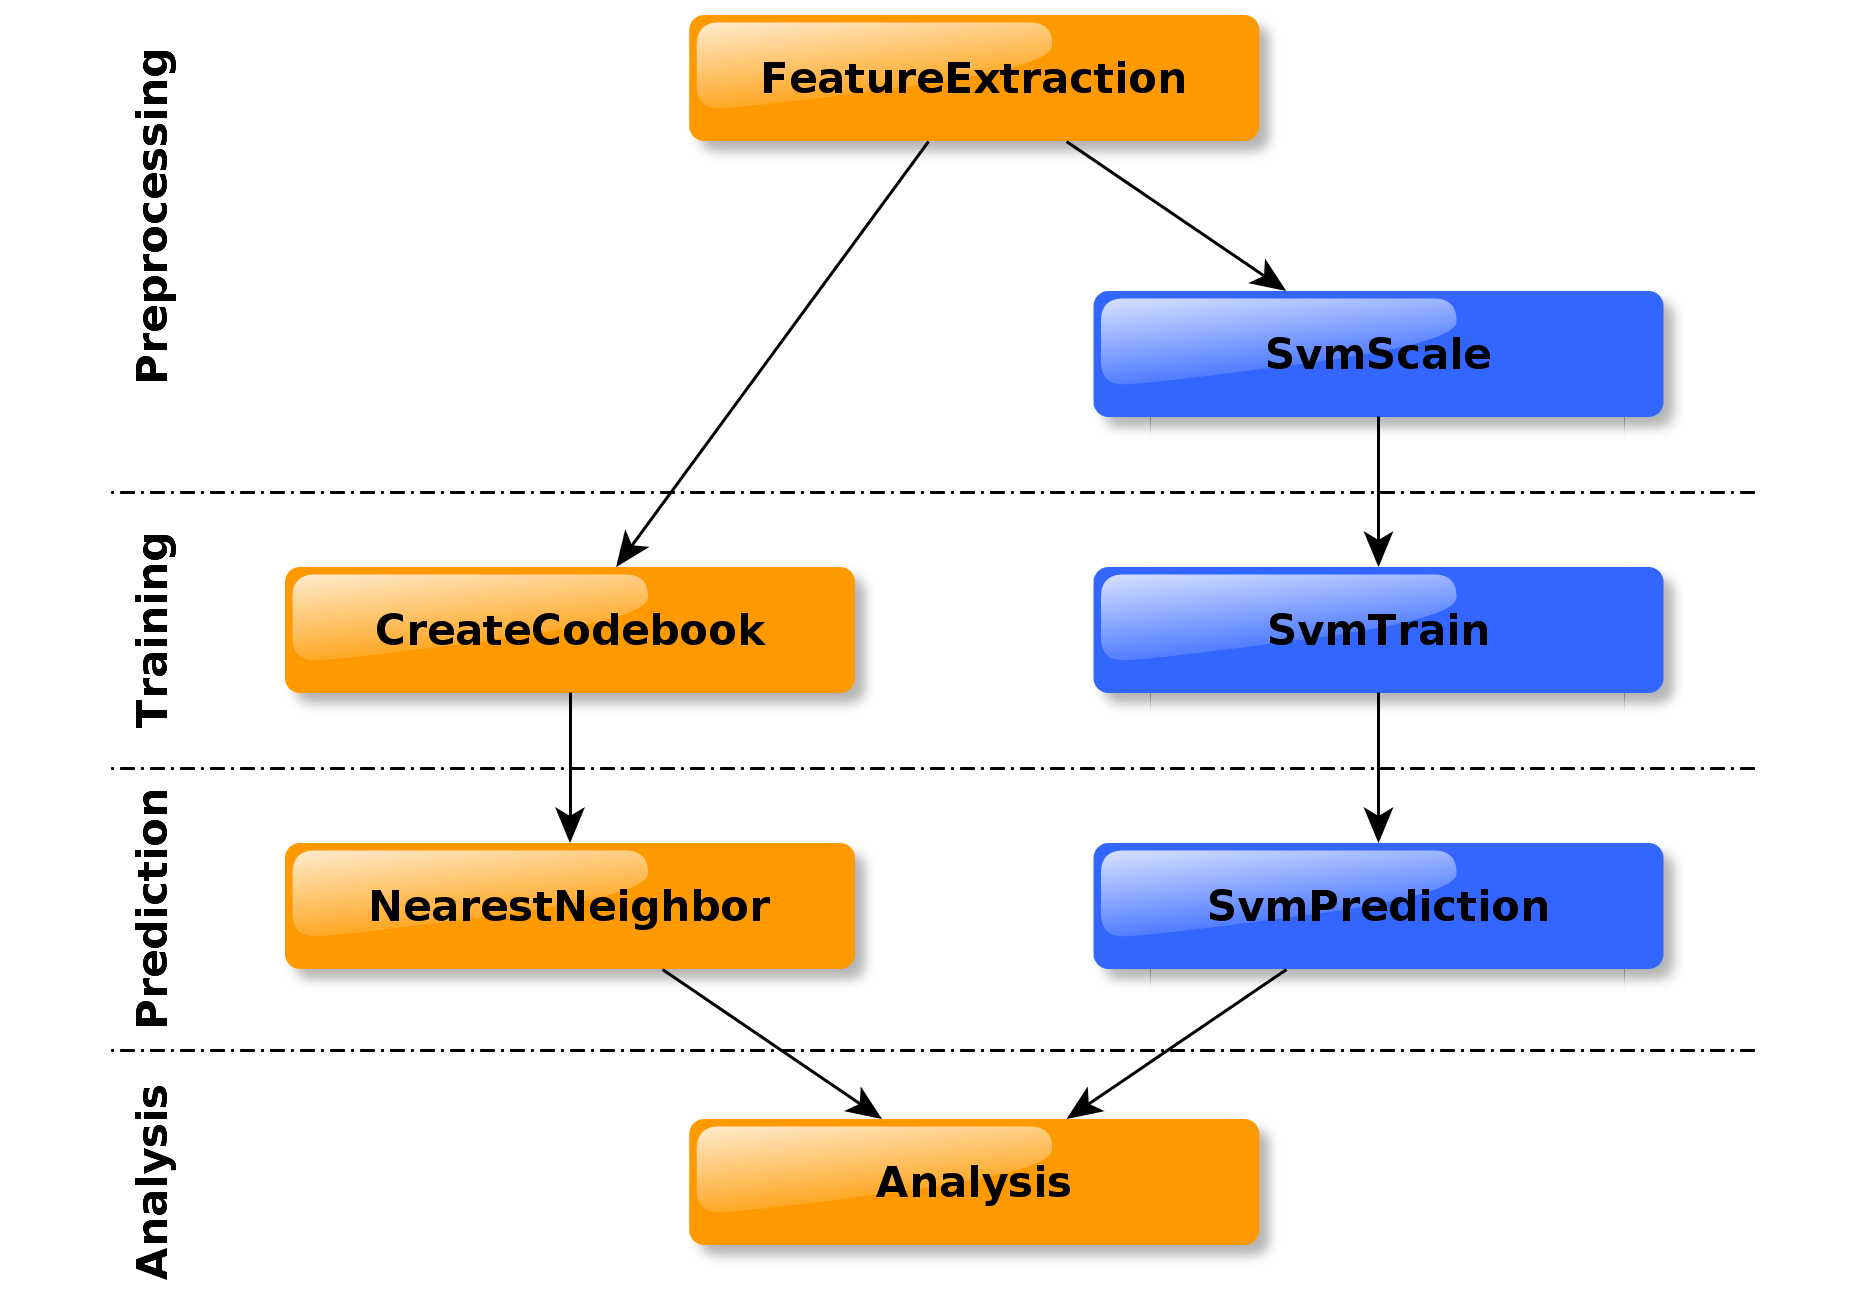
\includegraphics[width=1.0\textwidth]{img/moduluebersicht}
	\end{center}
\end{frame}

\subsection{Zusatz}
\begin{frame}{Zusatz}
	\begin{itemize}[<+->]
		\item Shell-Skript für Offline-Test
		\begin{itemize}[<1->]
			\item Kreuzvalidierung
			\item Sämtliche Einstellungen
		\end{itemize}
		\item Online-Modus
		\begin{itemize}[<1->]
			\item Nutzung der Offline-Module
			\item MFCC + Neural Gas
		\end{itemize}
		\item Evolutionärer Algorithmus
		\begin{itemize}[<1->]
			\item Optimierung
			\item MFCC + Neural Gas
		\end{itemize}
	\end{itemize}
\end{frame}
